\chapter{Statistics for particle analysis}
\label{chap:statistics}

\section{Classification functions}
\label{sec:classification_functions}

The main concepts which are used throughout the thesis heavily rely on statistical classification functions to compare the goodness of identification methods. However, their use is not limited to physics, let alone particle physics, but spans over all field containing some form of (binary) classification problem.
In the following paragraphs the examples assume one wants to identify kaons in a set of data containing a multitude of alternative particles. A classification into kaons and non-kaons is performed.

The most important classification functions are:
\begin{itemize}
	\item \textbf{T}rue \textbf{P}ositive \textbf{R}ate (\textbf{TPR}): \textit{proportion of accepted elements which are correct relative to all positives}

	\nobreak
	Hence, in the example it is the ratio of identified kaons which actually are kaons in proportion to the number of kaons in the data.

	\item \textbf{T}rue \textbf{N}egative \textbf{R}ate or Specificity (\textbf{TNR}): \textit{proportion of rejected elements which are incorrect relative to all negatives}

	\nobreak
	It is the ratio of non-kaon particles being identified as non-kaons in proportion to the number of all non-kaon particles.

	\item \textbf{F}alse \textbf{P}ositive \textbf{R}ate (\textbf{FPR}): \textit{proportion of accepted elements which are incorrect relative to all negatives}

	\nobreak
	The rate represents the fraction of non-kaon particles identified as kaons over the number of all non-kaons.

	\item \textbf{F}alse \textbf{N}egative \textbf{R}ate (\textbf{FNR}): \textit{proportion of rejected elements which are correct relative to all positives}

	\nobreak
	It is the fraction of kaons classified as being non-kaons over the number of all non-kaons.

	\item \textbf{P}ositive \textbf{P}redicted \textbf{V}alue (\textbf{PPV}): \textit{proportion of accepted elements which are correct relative to all accepted}

	\nobreak
	It represents the fraction of kaons classified as such over the number of all tracks classified as kaons but not necessarily being one.

\end{itemize}

In abstract terms: The two prefixes used above may be summarized as seen in \autoref{tab:classification_guidelines}. Bear in mind that \textbf{negative} and \textbf{positive} if used separately denote the presence of the desired feature and therefore do not fit the definition given in the table which is only for two word prefixes.

\begin{table}[ht]
	\centering
	\begin{tabular}{l|ll}
		& First word & Second word \\
		\hline
		Veracity & True = correct & False = incorrect \\
		Identification & Positive = accepted & Negative = rejected
	\end{tabular}
	\caption{Overview of prefixes used for classification function.}
	\label{tab:classification_guidelines}
\end{table}

\section{Receiver operating characteristic}
\label{sec:roc}

The \textbf{R}eceiver \textbf{O}perating \textbf{C}haracteristic (\textbf{ROC}) curve is the TPR plotted over the FPR. The values on the $x$ and $y$ axis go from $0$ to $1$. Each point on the seemingly continuos curve represents an applied selection criterion on the data or so called \textit{cut}.

A straight diagonal line connecting the point $(0, 0)$ with $(1, 1)$ would be the result of a classifier which is merely guessing the classes of two equally likely yields. A curve below this diagonal is worse than guessing and anything above is some degree of good. An optimal curve achieves a high TPR value at a very low FPR.
Multiple methods can therefore be compared by assessing the value and the slope of each methods TPR in dependence to the FPR. The \autoref{fig:sample_roc_curve} visually underlines the above described relations.

\begin{figure}[ht]
	\centering
	\includegraphics[width=\textwidth,height=0.4\textheight,keepaspectratio]{{{../res/Sample Receiver Operating Characteristic (ROC) curve}}}
	\caption{Sample ROC curve for a binary classification problem with each outcome being equally likely.}
	\label{fig:sample_roc_curve}
\end{figure}

Usually the leftmost points are of most interest as they represents a selection with only few false elements contaminating the sample.

\section{Identification efficiencies}
\label{sec:efficiency}

The identification efficiency is defined as the proportion of correctly classified particles of a class relative to all the available particles belonging to it. Hence, it directly represents the TPR. Both terms will be used as synonyms throughout the thesis.

The $\epsilon_{PID}$-matrix is the confusion matrix normed by row for an exclusive particle classification. The term `exclusive' in this context denotes that each track is labeled with exactly one particle hypothesis. Such a classification can be achieved by, e.g., assigning the track the label of the highest identification variable. This concept is used throughout the analysis.

Each cell in a row represents the probability of a particle of that row's class being identified as the particle of that column's class. The diagonal of the matrix contains the identification efficiencies for a particle species.

The definition generalizes to non-normed matrices, e.g., resulting from non-exclusive cuts. Although, reading the matrix is less intuitive as a particle might belong to multiple classes and comparing the values between different matrices becomes ambiguous.

The values of the matrix are given by the fraction of particles $i$ classified as $j$ over the true abundance of particle $i$. Hence, its values are

\begin{equation}
	\epsilon_{i j} = \frac{N_{i \text{ classified as } j}}{A_{i \text{ true}}}.
\end{equation}

The matrix has the shape of a $6 \times 6$ matrix when listing the confusion probabilities for all six particle species with an ID:

\begin{equation}
	\begin{pmatrix}
		\epsilon_{K K} & \epsilon_{K \pi} & \epsilon_{K e} & \epsilon_{K \mu} & \epsilon_{K p} & \epsilon_{K d} \\
		\epsilon_{\pi K} & \epsilon_{\pi \pi} & \epsilon_{\pi e} & \epsilon_{\pi \mu} & \epsilon_{\pi p} & \epsilon_{\pi d} \\
		\epsilon_{e K} & \epsilon_{e \pi} & \epsilon_{e e} & \epsilon_{e \mu} & \epsilon_{e p} & \epsilon_{e d} \\
		\epsilon_{\mu K} & \epsilon_{\mu \pi} & \epsilon_{K e} & \epsilon_{K \mu} & \epsilon_{K p} & \epsilon_{\mu d} \\
		\epsilon_{p K} & \epsilon_{p \pi} & \epsilon_{p e} & \epsilon_{p \mu} & \epsilon_{p p} & \epsilon_{p d} \\
		\epsilon_{d K} & \epsilon_{d \pi} & \epsilon_{K e} & \epsilon_{K \mu} & \epsilon_{K p} & \epsilon_{d d} \\
	\end{pmatrix}.
\end{equation}

In general, values on the diagonal should be close to $1$ while non-diagonal entries should vanish for a good classification approach. Bear in mind that the efficiency of a particle classification is always normed by the abundance of the particle and as such each row may have a different normalization. This is especially important when calculating the overall efficiency which is the fraction of all correctly classified tracks relative to all available tracks. In this case, each efficiency on the diagonal has to be weighted with the abundance of the particle specie.

\section{Likelihood}
\label{sec:likelihood}

\subsection{Likelihood ratio}
\label{subsec:likelihood_ratios}

The ratio of likelihoods is commonly used for comparisons of the goodness of different models. For each hypothesis a likelihood of event~$\pmb{x}$ occurring is calculated under the assumption the hypothesis is indeed true. The ratio of the likelihoods of two hypothesis $H_0$ and $H_1$
\begin{equation}
	\frac{\mathcal{L}(\pmb{x}|H_0)}{\mathcal{L}(\pmb{x}|H_1)}
\end{equation}
denotes how many times more likely the event $\pmb{x}$ is under hypothesis $H_0$ relative to $H_1$.

However, the event $\pmb{x}$ must not necessarily take the form of a simple one dimensional value. It may very well be a composition of, e.g., multiple detector responses. In case the components $x_i$ are independent from one another, one may simply construct the overall likelihood of $\pmb{x}$ by multiplying the separate likelihoods of each $x_i$. Hence, $\mathcal{L}(\pmb{x}|H_0)$ is composed out of multiple likelihoods each assuming $H_0$ to be true:
\begin{equation}
	\mathcal{L}(\pmb{x}|H_0) = \prod \limits_{i} \mathcal{L}_i(x_i|H_0).
\end{equation}
In case of event~$\pmb{x}$ being a detector response, the likelihood $\mathcal{L}(\pmb{x}|H_0)$ is the probability of measuring a signal given a particle hypothesis is true. Its value is constructed by multiplying the likelihoods of $\mathcal{L}_i(x_i|H_0)$ for each detector $i$.

\subsection{Neyman-Pearson}
\label{subsec:likelihood_ratios_neyman_pearson}

The Neyman-Pearson lemma is useful for evaluating the goodness of separating two models which have no unknown parameters. It states that a test on the likelihood ratio has the highest probability of correctly rejecting the original hypothesis if the alternative hypothesis is indeed true. In other words: A test on the likelihood ratio provides the highest purity at a given efficiency.

The purity of a selection is defined as the proportion of correctly classified particles relative to all the identified ones. Its definition is identical to the PPV and as such will be used as synonym throughout the thesis.

Hence, one expects to observe a monotonically increasing function by plotting the purity over the likelihood ratio. An idealized version of such a graph is depicted in \autoref{fig:neyman_pearson_visualization}. Since the underlying data may not be assumed to be a continues stream, the likelihood ratio has been binned as it better represents the actual shape to be expected.

\begin{figure}[ht]
	\centering
	\includegraphics[width=\textwidth,height=0.3\textheight,keepaspectratio]{{{../res/Neyman-Pearson Visualization}}}
	\caption{Visualization of a test on the likelihood ratio. Based on the Neyman-Pearson lemma one should expect an monotonically increasing function. Horizontal lines indicate likelihood ratio bins, while the line represents the overall trend and guides the eye. The pion likelihood relative to the other particle likelihoods is merely used to emphasize the connection to particle physics.}
	\label{fig:neyman_pearson_visualization}
\end{figure}

\section{Neural network}
\label{sec:neural_network}

An artificial neural network or simply neural network is a class of algorithms inspired by the central nerve system of biological beings. Instead of electrical signals being passed on from neuron to neuron with complex biological processes involved, an artificial neural network passes on numbers with functions representing neurons.

Despite only employing simplistic building blocks, a neural network is able to model any continues function arbitrarily well using one layer and an infinite number of neurons~\cite{NeuralNetwork:UniversalApproximation}. It is used in hopes of discovering hidden relations between variables and to utilize high dimensional correlations not otherwise obvious.

A simple approach is to stack multiple layers of neurons (\textit{nodes}) on top of each other and to connect the outputs of the previous layer with inputs of the new layer (feed-forward neural network). A network can be designed arbitrarily deep and provide a multitude of additional feedback loops (recurrent neural network) and further binning restrictions on node-inputs (convolutional neural network).

\begin{figure}[ht]
	\centering
	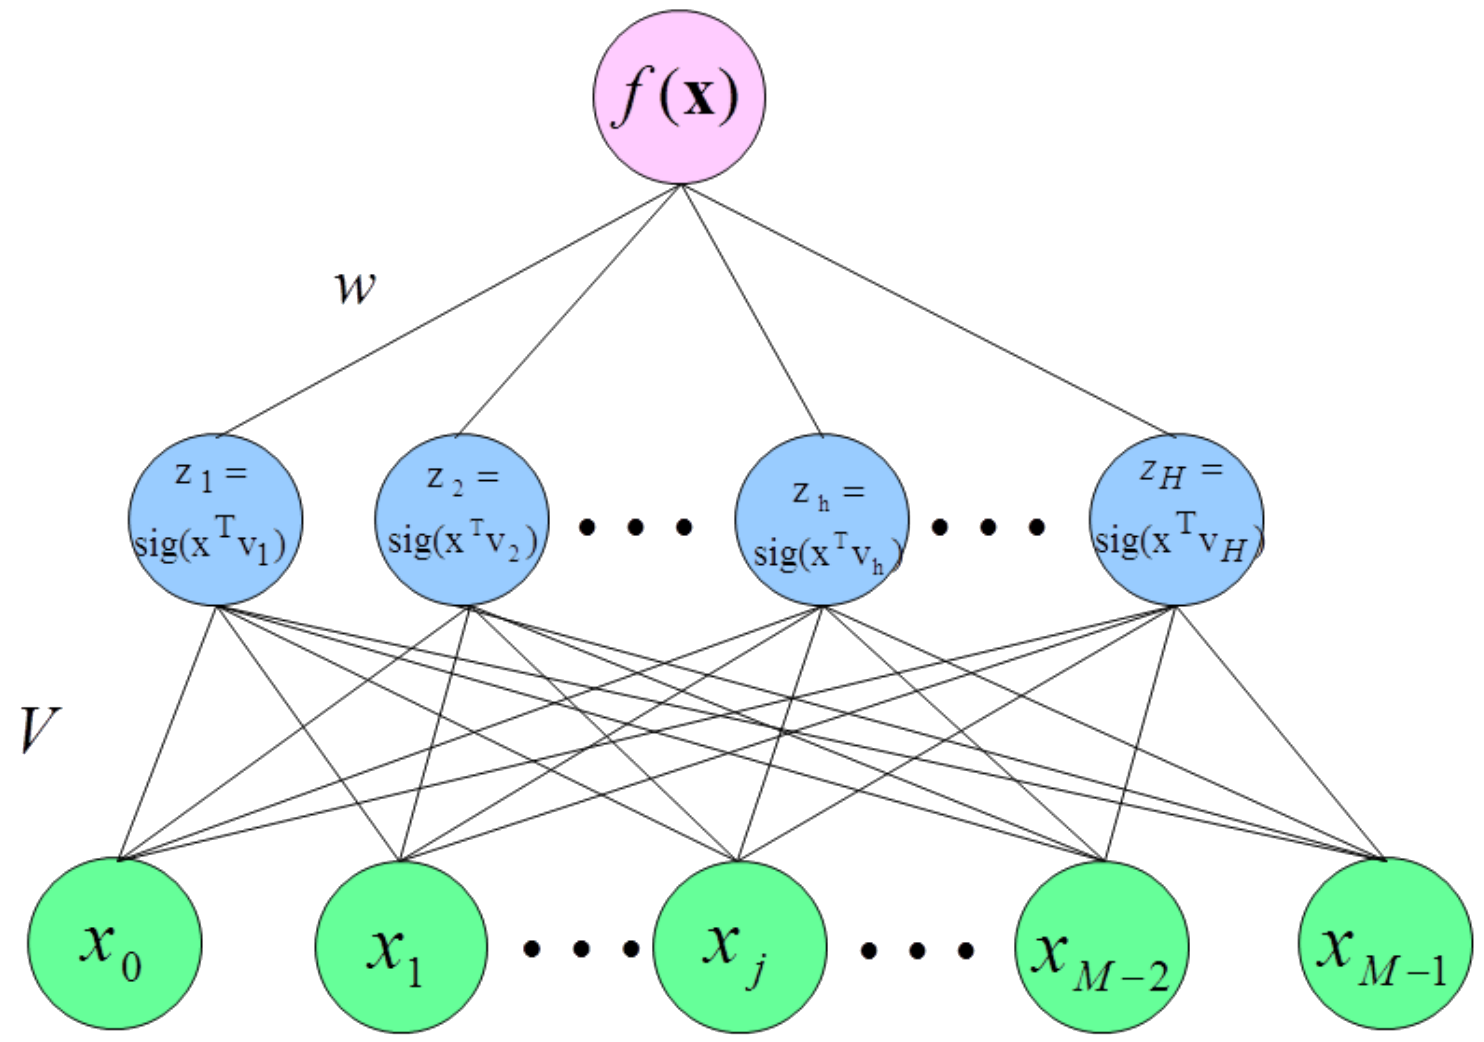
\includegraphics[width=\textwidth,height=0.4\textheight,keepaspectratio]{{{../res/Design of an artificial neural network}}}
	\caption{Design of an artificial neural network with one layer, $\pmb{x}$ as input, $z_i$ as activation function, $V$ und $w$ as weights and $f(\pmb{x})$ as prediction. Adapted from~\cite{MachineLearning:NeuralNetworks}.}
	\label{fig:sample_neural_network_design}
\end{figure}

A rather simple feed-forward network is depicted in \autoref{fig:sample_neural_network_design}. Each line between two bubbles represents a connection. In other words, the output of the bubble at the bottom is passed to the bubble at the top. The function used in calculating the various values of $z_i$ is called ReLU~\cite{MachineLearning:DeepLearning} and takes the form of $relu(h) = max(0, h)$. In terms of a biological system it can be though of as a boundary which has to be overcome prior to a signal being passed on.

Layers not representing the input or output are called hidden layers ({\color{blue}blue bubbles} from~\autoref{fig:sample_neural_network_design}). The dimensions of the input ({\color{green}green bubbles}) are also referred to as features. A function of a node is called \textit{activation function} ($z_i$). The term \textit{learning} in the context of neural network refers to the process of adapting parameters or so called \textit{weights} ($V$ and $w$) of a nodes via a gradient which optimizes the desired function. Often, the weights include a \textit{bias} which is a constant offset not influenced by any previous neuron. The desired function which is to be optimized is referred to as \textit{loss function}. It measures the predictive power of the classification. The job of the \textit{optimizer} is to adapt the weights in a way which minimizes the function, a task usually done via propagating the error back through the network in a schema called \textit{back propagation}. \textit{Training} in this context refers to the process of applying the network to a set of data and adjusting the weights as necessary for each iteration. The number of individual data points each iteration contains is described by the \textit{batch size}\footnotemark.

It is important to avoid making the network too dependent on the values in the training data. Otherwise it will simply \textit{over-fit} the given data without learning the more general concept. Meaning the neurons are perfectly adjusted to the input which it has already seen but the network fails upon receiving anything it has not already seen in this exact form.

\footnotetext{The last batch may be smaller if the total number of samples is not divisible by the batch size.}

Slight amendments are to be made for a multi-class classification problem. Namely a different activation function than the previously mentioned ReLU is used in the final layer. In this thesis the softmax algorithm is employed as last activation. Its response is given by
\begin{equation}
	P(c | x) = \frac{exp(x \cdot w_c)}{\sum \limits_{c' = 1}^{\#\text{classes}} exp(x \cdot w_{c'})}
	\text{,}
\end{equation}
with $c$ representing a class, $w_c$ the weights of a class and $x$ the input. The function assigns value between $0$ and $1$ to an element of belonging to class $c$. Note that the final output of the network is an exclusive classification into the class with the highest softmax value.

Additionally the loss function must be adapted to reflect the existence of more than two classes. In this study the categorical~cross~entropy~\cite{MachineLearning:LinearClassification} is chosen. In information theory, it puts a measure on the additional information needed to describe the data if deviating from the true underlying distribution.
